\documentclass[journal=jacsat,manuscript=article,layout=twocolumn]{achemso}
\usepackage[version=3]{mhchem} % Formula subscripts using \ce{}
\usepackage[T1]{fontenc}       % Use modern font encodings
% \usepackage[active]{preview}
%EXTRA PACKAGES%
% \usepackage{multicol}
\usepackage{xcolor}
\usepackage{textcomp}


%%%%%%%%%%%%%%%%%%%%%%%%%%%%%%%%%%%%%%%%%%%%%%%%%%%%%%%%%%%%%%%%%%%%%
%% Place any additional macros here.  Please use \newcommand* where
%% possible, and avoid layout-changing macros (which are not used
%% when typesetting).
%%%%%%%%%%%%%%%%%%%%%%%%%%%%%%%%%%%%%%%%%%%%%%%%%%%%%%%%%%%%%%%%%%%%%
\newcommand*{\ga}{\alpha}
\newcommand*{\gb}{\beta}
\newcommand*{\gam}{\gamma}
\newcommand*{\gd}{\delta}
\newcommand*{\eps}{\epsilon}
\newcommand*{\veps}{\varepsilon}
\newcommand*{\gz}{\zeta}
\newcommand*{\gt}{\theta}
\newcommand*{\gi}{\iota}
\newcommand*{\gk}{\kappa}
\newcommand*{\gl}{\lambda}
\newcommand*{\gs}{\sigma}
\newcommand*{\go}{\omega}
\newcommand*{\Gam}{\Gamma}
\newcommand*{\gD}{\Delta}
\newcommand*{\gT}{\Theta}
\newcommand*{\gL}{\Lambda}
\newcommand*{\gS}{\Sigma}
\newcommand*{\gO}{\Omega}
\newcommand*{\pt}[1]{\left( #1\right)}
\newcommand*{\pq}[1]{\left[ #1 \right]}
\newcommand*{\pg}[1]{\left\{ #1\right\}}
\newcommand*{\figref}[1]{\figurename~\ref{#1}}
\newcommand*{\red}[1]{\textcolor{red}{#1}}
\newcommand*{\blue}[1]{\textcolor{blue}{#1}}
\newcommand*{\gray}[1]{\textcolor{gray}{#1}}
% \renewcommand{\baselinestretch}

%%%%%%%%%%%%%%%%%%%%%%%%%%%%%%%%%%%%%%%%%%%%%%%%%%%%%%%%%%%%%%%%%%%%%
%% Meta-data block
%% ---------------
%% Each author should be given as a separate \author command.
%%
%% Corresponding authors should have an e-mail given after the author
%% name as an \email command. Phone and fax numbers can be given
%% using \phone and \fax, respectively; this information is optional.
%%
%% The affiliation of authors is given after the authors; each
%% \affiliation command applies to all preceding authors not already
%% assigned an affiliation.
%%
%% The affiliation takes an option argument for the short name.  This
%% will typically be something like "University of Somewhere".
%%
%% The \altaffiliation macro should be used for new address, etc.
%% On the other hand, \alsoaffiliation is used on a per author basis
%% when authors are associated with multiple institutions.
%%%%%%%%%%%%%%%%%%%%%%%%%%%%%%%%%%%%%%%%%%%%%%%%%%%%%%%%%%%%%%%%%%%%%
\author{Elizaveta Guseva}
\email{elizaveta.guseva@stonybrook.edu}
\affiliation[Stony Brook University]
{Laufer Center for Physical and Quantitative Biology, Stony Brook University, Stony Brook, NY, (United States)}
% \altaffiliation{A shared footnote}
\author{Ronald N Zuckermann}
\affiliation{Lawrence Berkeley National Laboratory (LBNL), Berkeley, CA (United States)}
\author{Ken A Dill}
\email{dill@laufercenter.org}
\phone{+1631 632 5400}
\fax{+1631 632 5405}
\affiliation[Stony Brook University]
{Laufer Center for Physical and Quantitative Biology, Stony Brook University, Stony Brook, NY, (United States)}


%%%%%%%%%%%%%%%%%%%%%%%%%%%%%%%%%%%%%%%%%%%%%%%%%%%%%%%%%%%%%%%%%%%%%
%% The document title should be given as usual. Some journals require
%% a running title from the author: this should be supplied as an
%% optional argument to \title.
%%%%%%%%%%%%%%%%%%%%%%%%%%%%%%%%%%%%%%%%%%%%%%%%%%%%%%%%%%%%%%%%%%%%%
\title[]
  {HP world model of early origin of biopolymers}

%%%%%%%%%%%%%%%%%%%%%%%%%%%%%%%%%%%%%%%%%%%%%%%%%%%%%%%%%%%%%%%%%%%%%
%% Some journals require a list of abbreviations or keywords to be
%% supplied. These should be set up here, and will be printed after
%% the title and author information, if needed.
%%%%%%%%%%%%%%%%%%%%%%%%%%%%%%%%%%%%%%%%%%%%%%%%%%%%%%%%%%%%%%%%%%%%%
\abbreviations{IR,NMR,UV}
\keywords{American Chemical Society, \LaTeX}

%%%%%%%%%%%%%%%%%%%%%%%%%%%%%%%%%%%%%%%%%%%%%%%%%%%%%%%%%%%%%%%%%%%%%
%% The manuscript does not need to include \maketitle, which is
%% executed automatically.
%%%%%%%%%%%%%%%%%%%%%%%%%%%%%%%%%%%%%%%%%%%%%%%%%%%%%%%%%%%%%%%%%%%%%



\begin{document}
\abstract{\footnotesize How living systems arose prebiotically from random physical-chemical 
processes is a
longstanding question. When did undirected(??) chemical reactions begin to capitalize on
fitness and undergo Darwinian evolution? 
Many origins-of-life studies are post-informational (postbiotic), i.e. focusing on
processes that happen after there is already a molecular code and an ability to
propagate ``self''.
Here, in contrast, we are focusing on the transition from prebiotic to postbiotic.
We are interested in how polymers with random sequences may lead to informational
polymers with particular sequences, which then dominate the population. To study
sequence-structure properties of informational copolymers we use HP lattice model --
a successful polymer-folding model of hydrophobic (H) and polar (P) monomers. 
Using sequences and structural information from the HP-model we have found
conditions under which a set of certain sequences dominates the population with time.
We use direct stochastic simulations of the dynamic models of the polymerization to
figure out how sequence structure and aspects of the different dynamic models
determine the structure and behavior of the emerged cooperative sets of the
polymers. We find that some sequences become autocatalytic for accelerating the
syntheses of others.}

%%%MAIN TEXT%%%%

 
\section{Introduction} 

% Functioning of modern organisms is not possible without nucleic 
% acids and proteins. Cells produce these extremely long polymers with complex cell machinery 
% like ribosomes and polymerases -- also extremely long polymers. 
% Therefore question ``how long polymers can be produced prebiotically?'' is crucial for the origin 
% of life research whether one's approach is information first or metabolism first.
Two important puzzles in understanding the early origins of life are: how prebiotic polymerization 
processes could have produced long chains of protein-like or nucleic acids-like molecules, and how 
information molecules could have arisen from random sequences.
While we know that amino acids can be produced prebiotically \cite{Miller1953} and are abundant in 
stony meteorites \cite{Sephton2002} and significant progress has been made in synthesis of 
single nucleotides \cite{Powner2009a}; a discovery of a mechanism of prebiotic 
production of biochemically long polypeptides or nucleic acids despite certain success, is 
 still in the future, and chains obtained non-enzymatically are typically short 
\cite{Shock1992,Martin1998,PAECHT-HOROWITZ1970,Lambert2008,Leman2004a,Orgel2004,Ferris1996}.

Several mechanism were proposed to increase yields of oligomers: adsorption to 
clays\cite{Rao1980,Lambert2008}, minerals\cite{Bernal1949,Ferris1996}, evaporation of tidal 
pools\cite{Nelson2001}, concentration in ice through eutectic melts \cite{Kanavarioti2001}, 
freezing conditions\cite{Bada2004} or temperature cycles. 

However the main problem with spontaneous polymerization processes is that it falls under what we 
call Flory problem: chain length distribution has an exponential asymptote, and desirably long 
chains are present in negligible quantities.

Maximum length of biopolymers reached (both nucleic acids and peptides) in the lab 
during non-enzymatic synthesis range from 2-3mers to 
55\footnote{primary product contains 20-40-mers, mean chain length is expected to be 
30\cite{Ferris1996}} monomers long depending on conditions and initial length of substrate.  

Rode et al.\cite{Rode1997,Rode1999} used various mineral catalysts such as calcium 
montmorillonite, hectorite,  silica, alumina for elongation mixture of Gly and Gly$_2$ at 
40\textcelsius\, got sequences up to length 6 after 14 reaction days.

Ferris et al.\cite{Ferris1996} got sequences up to length 55, with most of the product being 
20-40mers. They started from decanucleotide [$^{32}$P]dA(pdA)$_8$pA adsorbed on 
Na$^+$-montmorillonite and daily added ImpA. After 14 days at 25\textcelsius\, primary product 
contained 20-40mers with some sequences exceeding 0-5mers.

Kanavarioti et al.\cite{Kanavarioti2001} got oligouridylates up to 11 bases long with average 
value of 4. They froze samples of phosphoimidazolide-activated uridine to react at 
-18\textcelsius\, in the presence of metal ions in dilute solutions.

Thermodynamics of aqueous solutions
normally doesn't allow for any significant quantities of oligo-peptides to be formed, even 2-3mers.
Leman et al. \cite{Leman2004a} Showed thatcarbonyl sulfide (COS), a simple volcanic gas, brings about the
formation of oligo-peptides from amino acids under mild conditions in aqueous
solution. They got up to 80\% yields of oligo-peptides in minutes to hours at room temperature.
While product is 2-3mers with most of the product being 2-mers. Experiments are performed in 25\textcelsius,
with pH varied between 5.9 and 9.8.


Some representative data is shown on fig \ref{fig:some_flory} along with fitted Flory-Schulz 
distributions.
\begin{figure}[h!]
  \centering
  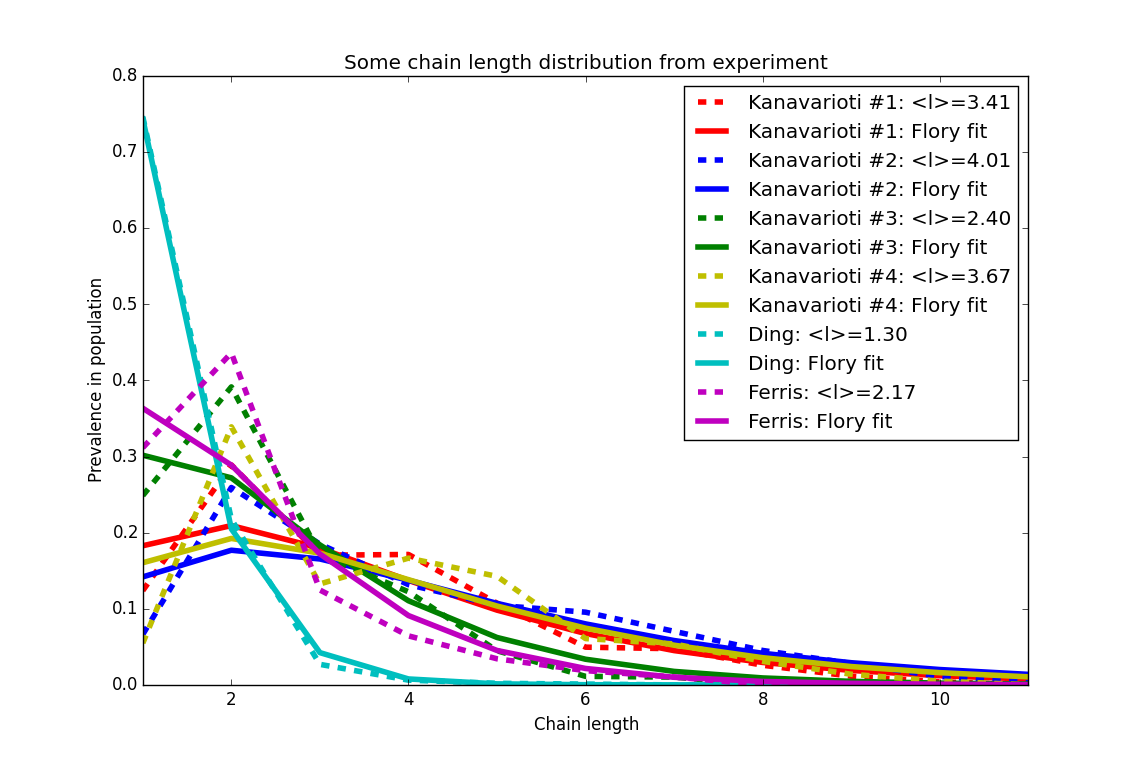
\includegraphics[width=\columnwidth]{pictures/some_flory.png} 
  \caption{Experimental results from \cite{Kanavarioti2001} and their fitting to Flory 
distribution. Data points: Kanavarioti\cite{Kanavarioti2001}, Ding\cite{Ding1996}, 
Ferris\cite{Ferris1999} }
  \label{fig:some_flory}
\end{figure}



This suggests that first catalysts emerged from mixture of short sequences, which were both 
not diverse and had poor information content. Therefore the problem of short chains also brings 
with itself problems of information production and complexity emergence \cite{Joyce1987,Abel2005}

 We sought a simple structure based mechanism, 
which would solve Flory problem, which would be able to select for certain sequences and 
amplify their chain lengths.

 We present here a physical mechanism, which give rise to 
heavy tail chain lengths distribution and selects the sequences based on the physical principle: 
hydrophobic interaction. Our mechanism doesn't have to be the only one. It can be successfully 
applied if there another accelerating processes such as adsorption or wetting and drying cycles, 
for example.
% \red{write about autocatalytic sets here and cite Kauffman, maybe also mention far from 
% equilibrium statement. mention composomes, mention lipid vesicles \cite{Luisi1999,Deamer2008}}
Our \textit{in-silico} experiments demonstrate that binary polymers 
capable of primitive folding and hydrophobic interaction is a working mechanism. Not only we get 
longer chains and selection. Our systems gives reasonable computational diversity of the sequences.

While our mechanism is an implementation of an autocatalytic process, such as for example 
introduced in \cite{Kauffman1986}, in addition to autocatalysis itself it provides a simple 
physical non-linear relation between sequence of polymer and its catalytic/substrate abilities, 
therefore giving an opportunity to experimentally test \red{\textbf{Something more about 
experiments, connection to Ron's lab??}}

   
\section{The ``Flory problem'' of obtaining long chains}
\label{sec:flory} 
The Flory or Flory-Schulz distribution describes the relative ratios of polymers of different 
lengths after a polymerization process, based on their relative probabilities of 
occurrence\cite{Flory1953}. 
\begin{equation}
 f(a)=a^2l(1-a)^{l-1},
\end{equation} 
where $l$ is a chain length and $a$ is an empirical 
constant, which is related to the average chain length: $\bar l = a(2- a)$
Figure \ref{fig:flory} represents Flory distribution  with different average chain length. 
This distribution gives the following polymer abundance for the blue line:
\begin{equation}
  \frac{\pq{10mers}}{\pq{1mers}}\propto10^{-4},\qquad\frac{\pq{20mers}}{\pq{1mers}}\propto10^{-9}
\end{equation} 
For such a system, if we start with nano-molar concentrations of monomers, 40-mers will have 
concentrations $\propto 10^{-23} $ mol/L, which is just a few molecules per liter. 
\begin{figure}[h!]
  \centering
  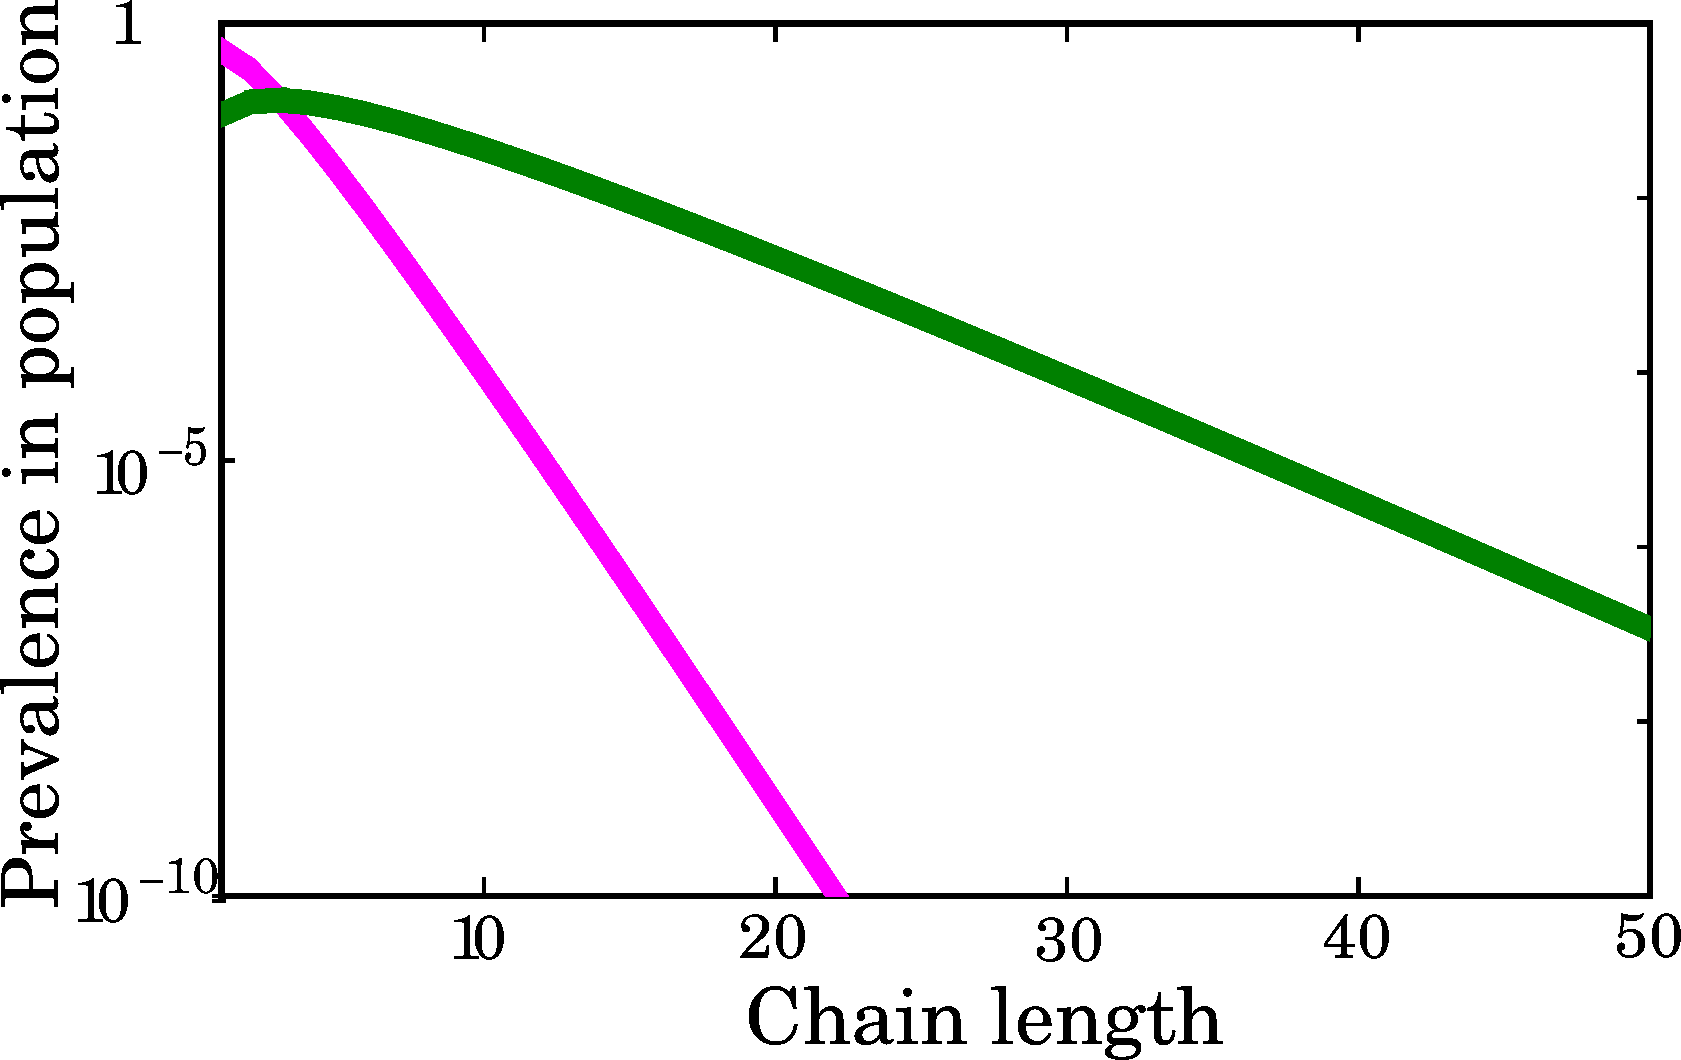
\includegraphics[width=\columnwidth]{pictures/flory2.pdf} 
  \caption{Spontaneous polymerization gives Flory length distribution with exponential asymptote.}
  \label{fig:flory}
\end{figure}

 While increasing equilibrium constant by means of catalysis or 
changing conditions to dry medium would lead to longer chain lengths, it will still give 
exponentially decreasing distribution of length. The proof for polymer concatenation is present 
in \cite{Derr2012}. This dynamics can be observed even in some autocatalytic systems \cite{Wu2009}.

The problem is that in the systems with spontaneous polymerization distribution of chain lengths 
of the produced polymers has an exponential asymptote  (see fig. \ref{fig:flory}). Depending on the 
actual system it can can follow for example actual exponential 
law  $f(a)\propto a^l$\cite{nowak2008prevolutionary,Derr2012} or a Flory distribution 
$f(a)=a^2l(1-a)^{l-1}$\cite{Flory1953}.
In either case, given low prebiotic concentrations of amino acids and nucleotides with estimations 
of submillimolar to submicromolar\cite{Aubrey2009,Kanavarioti2001,Lazcano1996}, longer chains 
would not be observable.



\section{Foldable polymers can help solving Flory problem}
We suggest that random synthesis of foldable polymers can lead to longer chains that carry 
information.
Here we propose a model of prebiotic synthesis of foldable polymers, such as proteins or RNAs, 
using the HP lattice model\cite{lau1989lattice,Chan1991,Miller1995,Yue1995,agarwala1997local}. The 
HP model supports two types of monomers: H (hydrophobic) and P (polar). It has been used 
extensively to study sequence-structure relationship in protein-like molecules. HP model has a 
folding code: presence of hydrophobic interaction makes some conformations 
of the same chain more energetically favorable than others. Moreover certain chains will have a 
unique conformation, which delivers free energy minimum. This conformations are called native 
states, and sequences, which have native state, are considered being capable of folding (see fig. 
\ref{fig:hydro-effect} ).

\begin{figure}[h!]
  \centering
  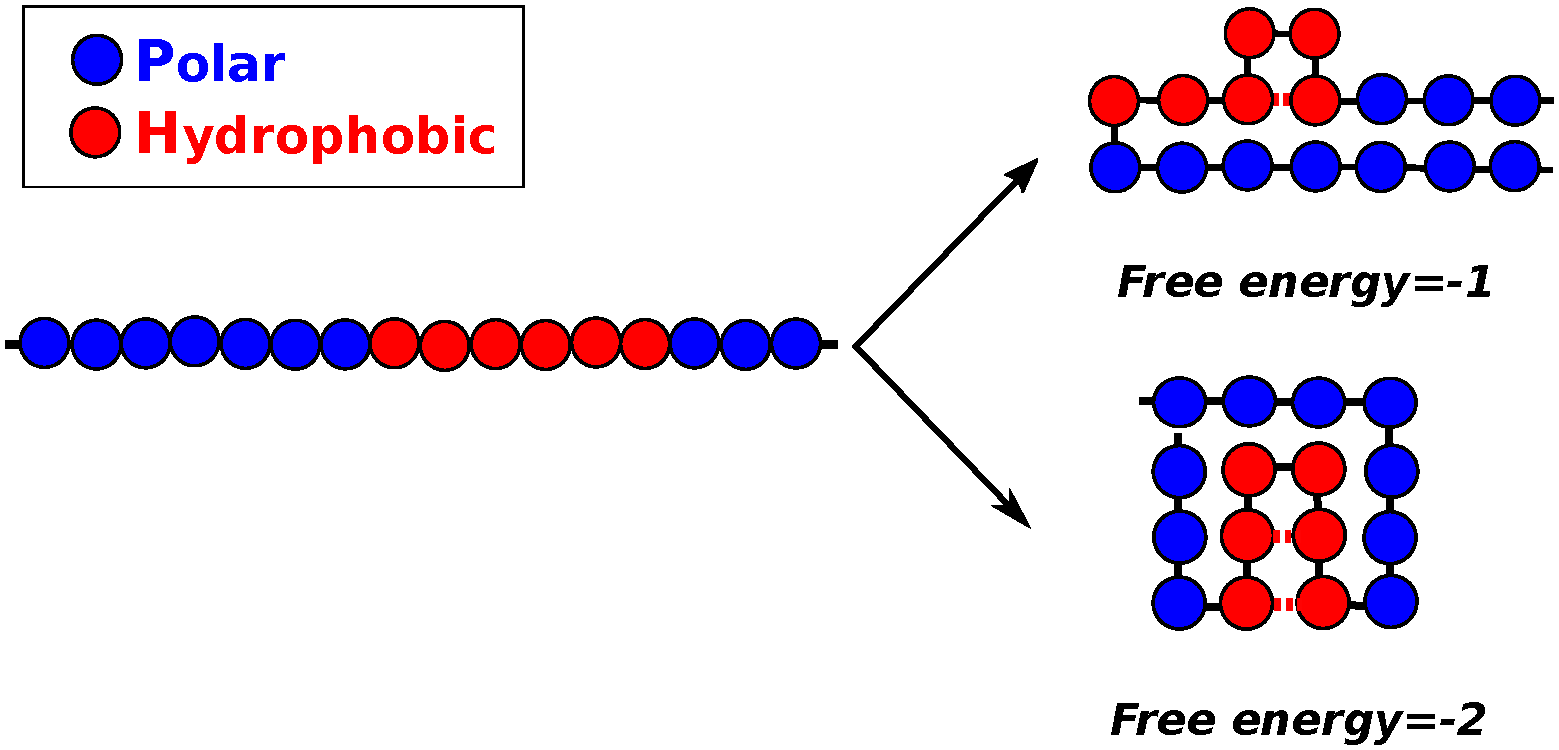
\includegraphics[width=\columnwidth]{pictures/hp-model.pdf} 
  \caption{HH-pairs are favorable in water. Interaction between them lowers free energy $\gD G$ of 
the chain, allowing for some conformations to get stability.}
  \label{fig:hydro-effect}
\end{figure}

Because of the ability to form hydrophobic contacts in water, even hetero-polymers that 
are as simple as HP-polymers will often fold up, even as short chains. 
While short HP chains will not necessarily have great stability qualities (they will often be 
fairly amorphous ``oil-drop''-like balls that are ensembles of conformations), some HP 
sequences will fold uniquely. They will spend most of the time in this unique state with the 
lowest free energy -- native state. And, what is important, it has been shown that a 
relatively large fraction of sequence space will fold to compact structures or compact ensemble 
structures\cite{lau1989lattice}.

\subsection{Some HP-foldamers may also be prebiotic catalysts}
Our central premise is that the same promiscuous hydrophobic interactions that can cause random 
HP heteropolymers to collapse into compact, folded, structures. However hydrophobic 
interaction will also cause polymer-polymer attraction and binding between molecules.  In some 
cases, a folded HP-polymers can provide a hydrophobic ``landing site'' for another HP polymer 
and/or another H monomer (see fig. \ref{fig:hp-catalysis}).  


When a folded chain has exposed hydrophobic monomers on its surface it can attract another chain 
with hydrophobes as well as activated hydrophobic monomer. Interaction between 3 of them localizes 
growing chain and next monomer (fig.\ref{fig:hp-catalysis}(a)). In addition to that, hydrophobic 
interaction also lowers activation barrier of the polymerization reaction, accelerating reaction 
this way.

One hydrophobic interaction is about $1-2kT$. Given that rate of catalysis is proportional to an 
exponent of the activation barrier, 3-4 hydrophobic interactions are enough to increase 
polymerization rate $\approx 100$ times (fig.\ref{fig:hp-catalysis}(b)). 
Of course, this is not a good rate enhancement, compared to $2\cdot10^7$-fold rate enhancement 
brought about
by modern ribosomes\cite{Sievers2004a}. However the very 
first catalysts don't have to be very efficient: their purpose is to create a driving force of 
evolution.

HP-catalysis drives addition of hydrophobes to hydrophobes. A seemingly logical conclusion would 
be that one will end up with purely hydrophobic polymers. However this is not true. Sequences 
capable of catalysis must have a relatively stable structure. Purely hydrophobic sequences don't 
have this property: they have very many conformational states with the same low free energy. 
Therefore they will spend a lot of time jumping between those states and their bonds will be 
affected by hydrolysis. They also will not be able serve as catalysts. Sequences with $50-80\%$ 
of hydrophobes, on the other hand, will have the most stable structures; they will 
be protected from hydrolysis and will be able to localize growing chain with the next added 
monomer.
\begin{figure}[h!]
  \centering
  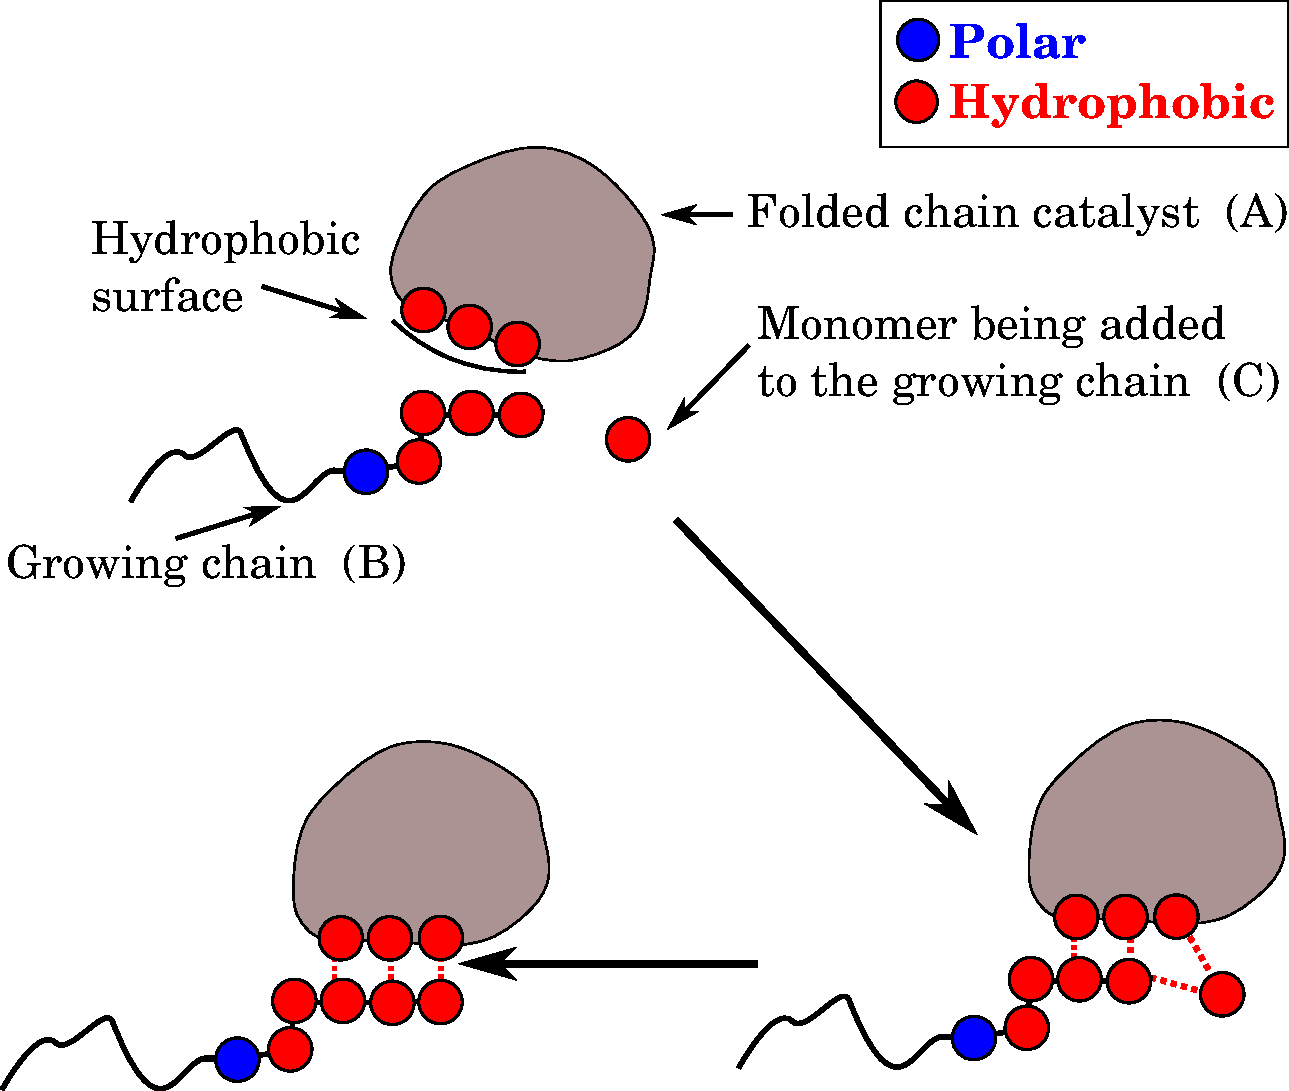
\includegraphics[width=0.9\columnwidth]{pictures/hp-catalysis.pdf} 
  \caption{Catalyst catalyzes a growing of an unfolded hp-polymer. 
           Having just 3-4 hydrophobic contacts is enough to lower an 
           activation barrier for $\propto 100$ times at room 
           temperature.}
  \label{fig:hp-catalysis}
\end{figure}







\section{Results}\label{sec:res}
\paragraph{Simulation: folding.} Presence of folding reactions and absence of catalysis ones 
relationship between abundance and length at steady state follows exponential distribution for 
longer chains and is slower than exponential for short chains. While presence of folding makes 
some of the folded sequences get higher than average for their length populations, these 
populations are never more than few-fold of average population of regular sequences and don't 
change nature of the distribution.
\begin{figure}[h!]
  \centering
  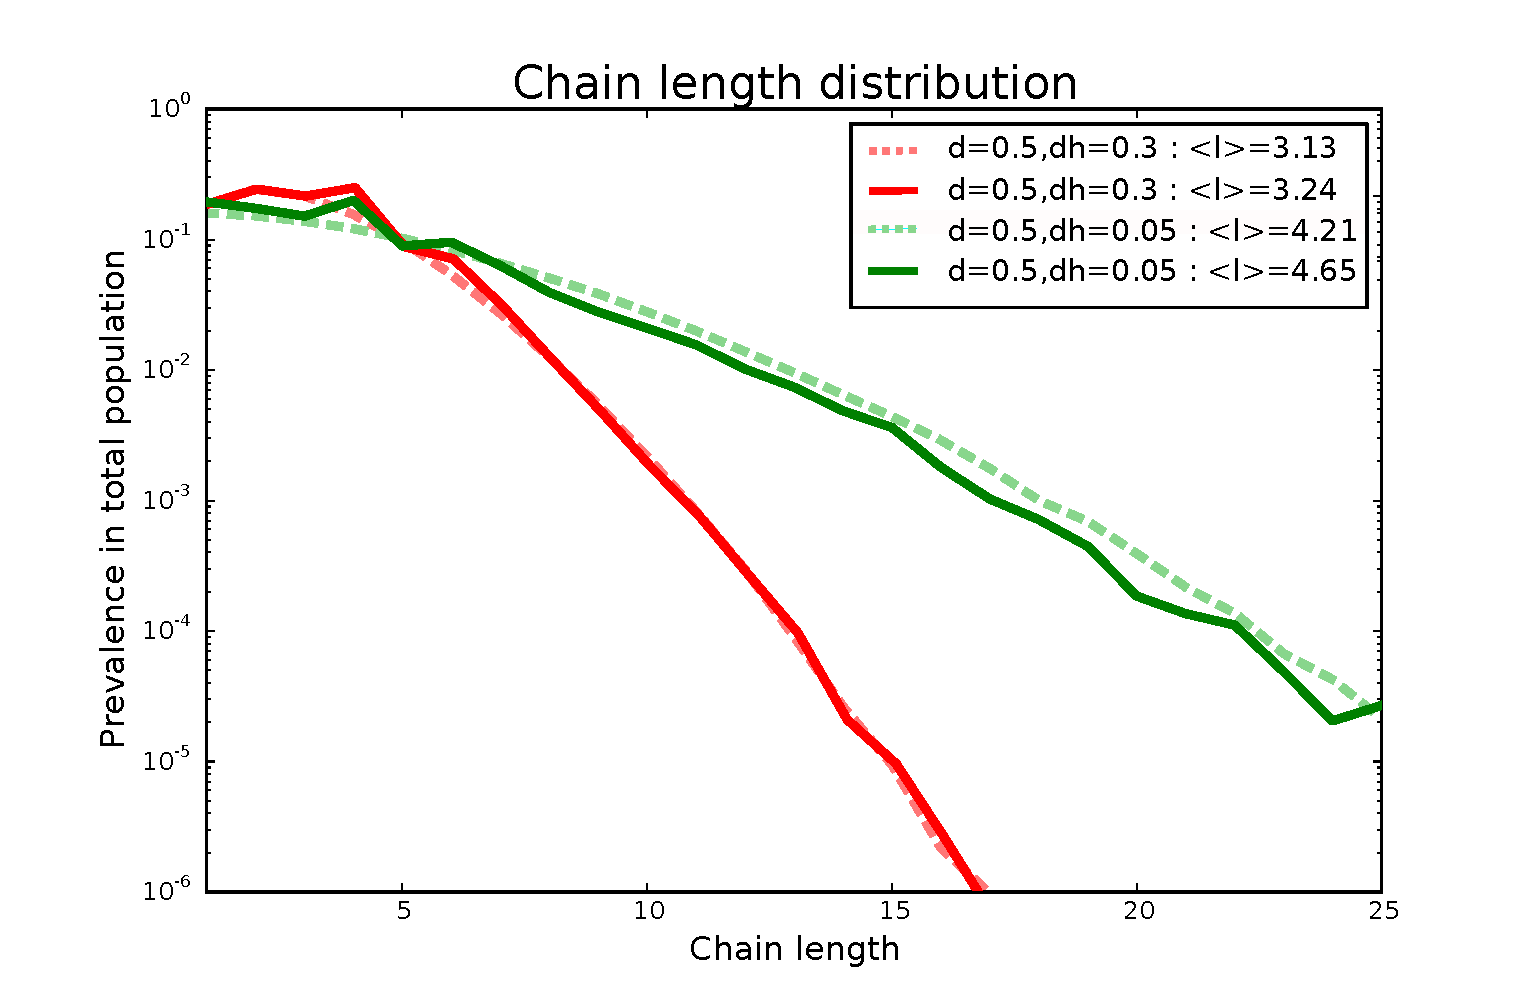
\includegraphics[width=\columnwidth]{pictures/flory-and-fold.pdf} 
  \caption{Dashed lines represent polymerization without folding or catalysis. Solid lines 
correspond to simulations run with folding but without catalysis. For details of simulations see 
section \ref{sec:mat-sim}, Experiment 2. }
  \label{fig:sim.flory-fold}
\end{figure}

\paragraph{Simulation: folding and HP-catalysis.}Presence of catalysis in the system skews the 
distribution significantly, and while it leaves average chain length about the same it brings 
substantial excess of long sequence compared to the cases without catalysis\ref{fig:sim.flory-hp}. 
The system is fairly stable towards hydrolysis and dilution parameters. It allows for 1 order of 
magnitude change in those parameters without significant change in the behavior of the system. 
Sequences responsible for the skew of the distribution are few in numbers they all are catalysts 
and have long stretches of hydrophobes, which also means that they are products of catalysis. In 
the figure \ref{fig:example1} there examples of several sequences. The lines represent average 
over 30 time evolutions. For this particular experiment, concentration of monomers at steady 
state is $\propto 100$. Most of the longer sequences have average populations $\ll 1$. However for 
the most of the chain lengths there are few sequences, which dominate populations significantly.
\begin{figure*}[h!]
  \centering
  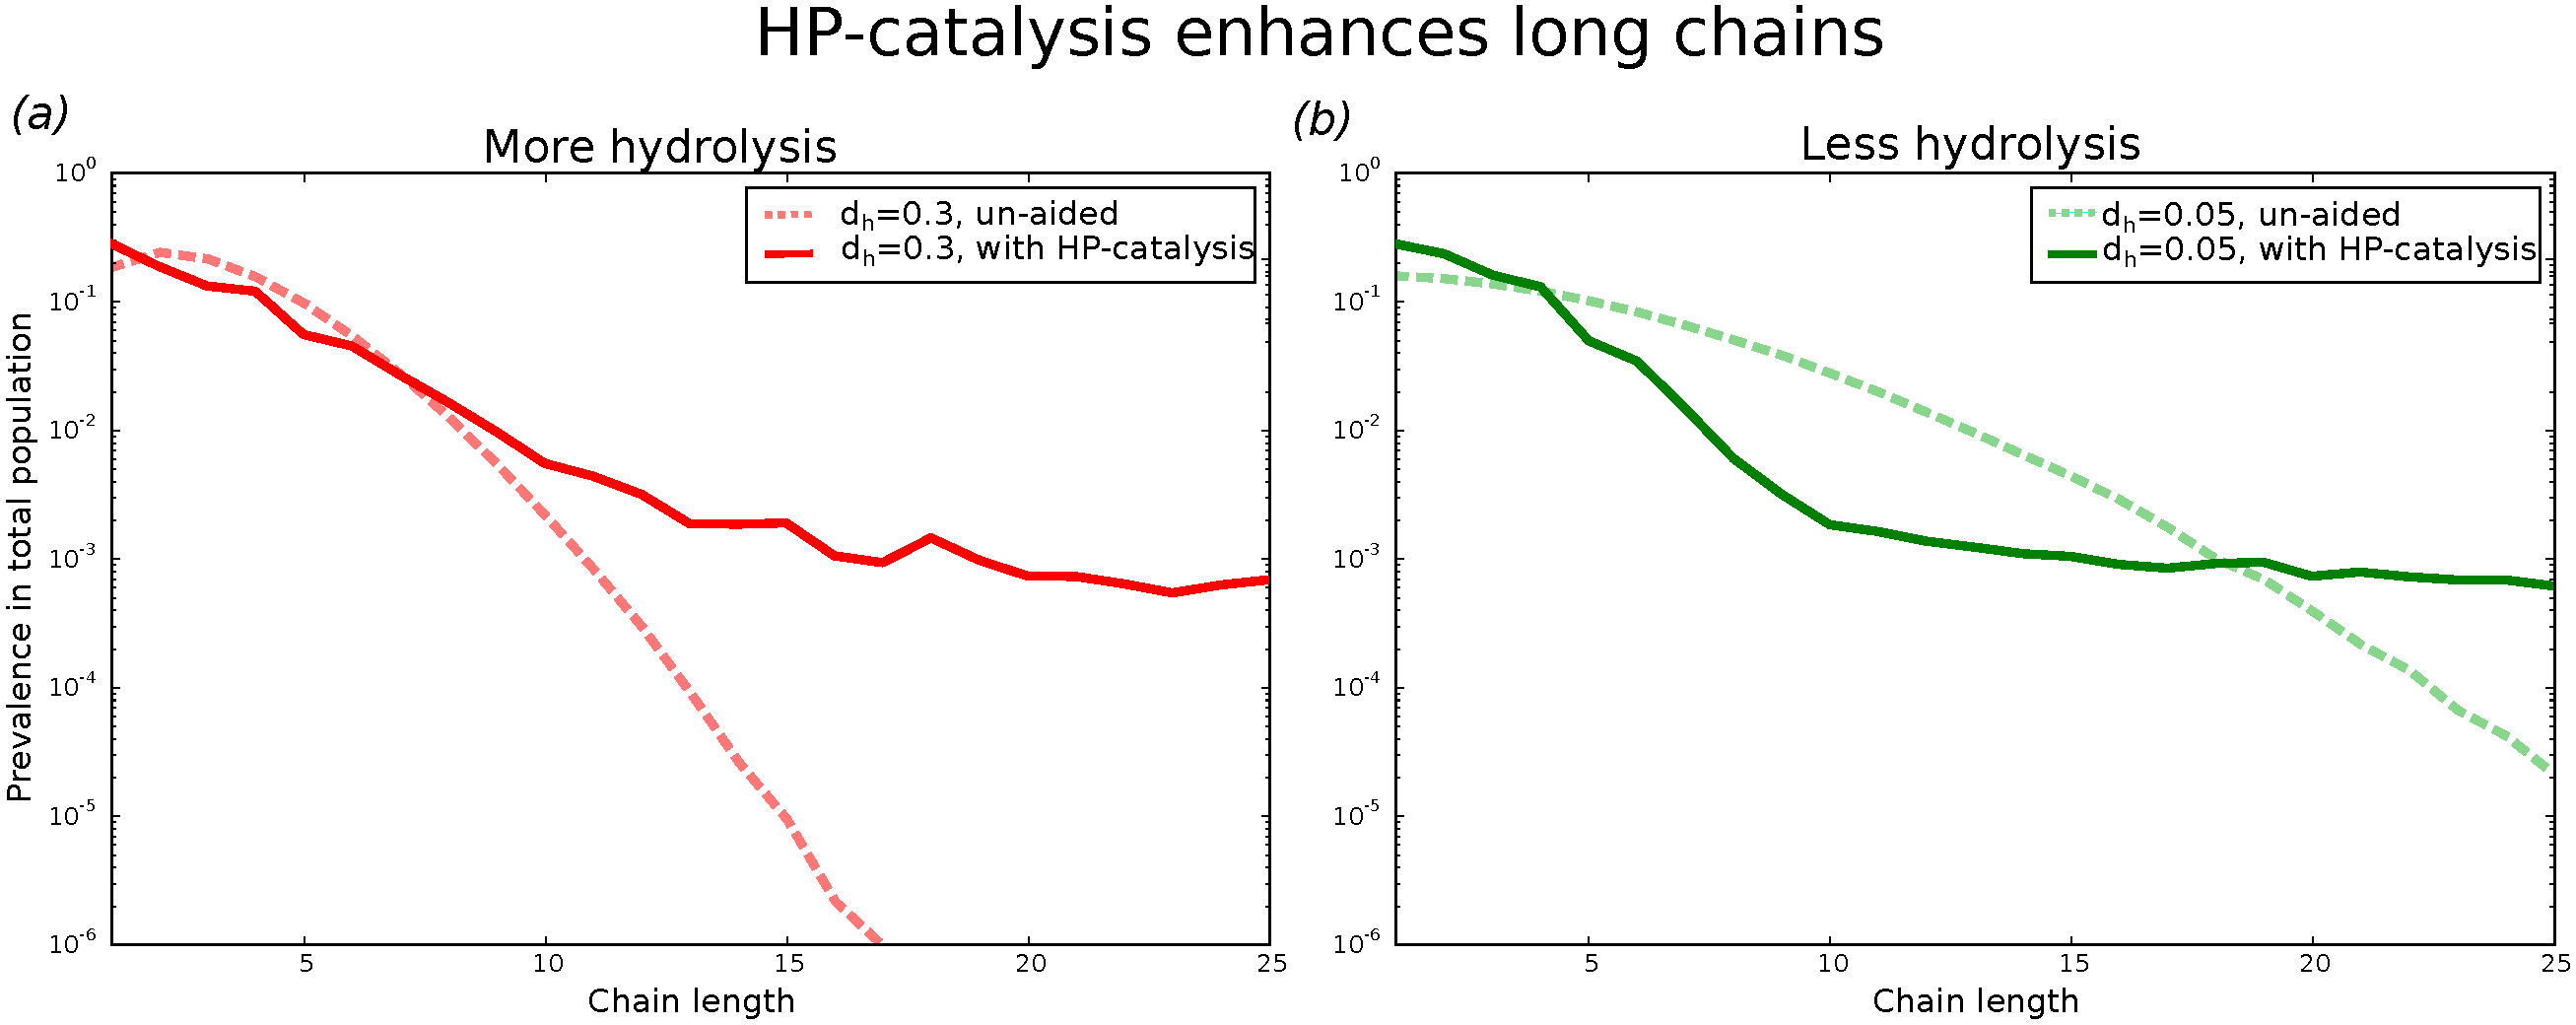
\includegraphics[width=0.95\textwidth]{pictures/flory-and-hp.pdf} 
  \caption{Dashed lines represent polymerization without folding or catalysis. Solid lines 
correspond to simulations run with folding and catalysis. For details of simulations see 
section \ref{sec:mat-sim}, Experiment 2. }
  \label{fig:sim.flory-fold}
\end{figure*}
\begin{figure}[h!]
  \centering
  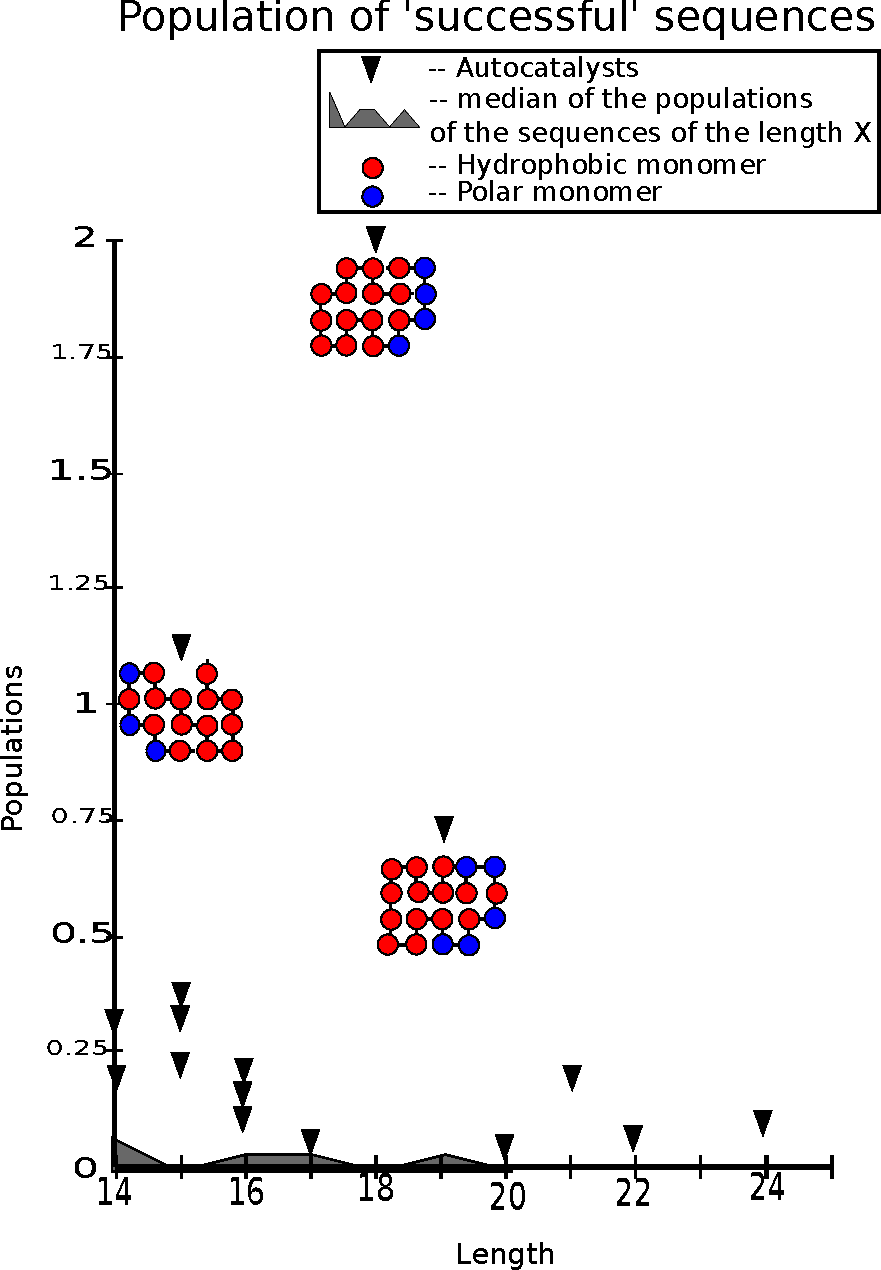
\includegraphics[width=\columnwidth]{pictures/good_seqs.pdf} 
  \caption{Some examples of dominating autocatalytic sequences. Gray lines represent regular 
non-catalytic sequence. structures on the right are native structures of autocatalytic sequences. }
  \label{fig:example1}
\end{figure}
\,\\
\.\\
\,\\
\,\newline\\


\section{Discussion}

\subsection{Autocatalysis}
Withing networks of chemical reactions of living systems there are many interactions and 
inter-dependencies. They make final systems functionally closed and self-sustaining, when out of 
available resources system produces whatever chemical components it needs. However probability of 
emergence of such a system out of mixture of simple molecules is essentially zero, and question of 
how it's possible, bothers many minds. Because functional closeness and self-maintenance are 
prominent properties of life significant amount of research since 1970s was focused on 
autocatalytic sets -- collections of entities, each of which can be created catalytically by 
other entities within the set, such that as a whole, the set is able to catalyze its own production.

This notion of an autocatalytic sets became popular in the origins of life community due to 
several reasons. To mention a couple:
\begin{enumerate}
 \item First, autocatalysis is a powerful mechanism, which 
produces complex dynamics: in all known chemical systems bi-stability, oscillations or generation of 
waves can be 
explained by one chemical mechanism, and at least one stage of it must be 
autocatalytic\cite{Prigozhin1990}. Production 
of physical-chemical complexity is one of the steps towards discovering origin of life. 
\item Second, autocatalysis seems to be 
a natural way to increase naturally extremely low yields of oligomers produced non-enzymatically and 
get an 
exponential growth, which is necessary for efficient self-replication.
\end{enumerate}

  In our analysis of a polymerization prebiotic systems we applied a physical principle of 
hydrophobic interactions to this old idea  of autocatalytic sets \cite{Kauffman1986,Eigen1978}. 


Here are some examples of other models using autocatalytic sets
\begin{itemize}
 \item Several studies\cite{Eigen1978,Dyson1985,Kauffman1986} focused on how such self-sustaining 
systems could work if they already exist. They investigated under which conditions these systems 
indeed are self-maintaining.

\item In a more recent series of works \cite{segre1998graded,Segre2000,Markovitch2012} 
 authors numerically studied auto and cross catalysis in an artificial chemical system of 
 small mutually catalyzing  molecules. They found parameters of the system for which one can observe 
diversity and replication fidelity.
 Appearance of these desirable properties requires high mutual catalysis propensity.

\item In \cite{Tkachenko2014} authors studied random heteropolymers capable of template 
assisted ligation and random breakage. In such a system, they showed,  long-chained
polymers  can be sustained by the mutual catalysis of the ligation reaction. They discovered
that a system with ligation and hydrolysis is capable of first order phase transition, depending concentration. 
In their system the maximum length of heteropolymers is determined kinetically as a simple function of the ratio
between ligation and breakage rates

\item In \cite{Walker2012} authors considered a system with finite monomer source, spontaneous reversible polymerization
and template ligation of binary polymers. With stochastic simulations, they studied how kinetic rates of polymerization/degradation
affect ability of sequences to explore sequence space. Similarly to our results, the higher the ratio of degradation rate
over polymerization rate (in our case (hydrolysis and hydrophobic energy), the higher the diversity 
of the pool, and the lower it, the higher number of functional sequences is observed (functional polymers are randomly assigned). Functional sequences are able to emerge spontaneously,
they don't dominate the pool, allowing for further pool exploration. While \cite{Walker2012} and our system are kinetically different they experience rather similar dynamics.
\end{itemize}

Many studies focused on how in a particular situation autocatalytic systems could arose and on 
different properties of the emergent results based on type of autocatalytic mechanisms.
\begin{itemize}
\item The idea of 
autocatalysis was applied by Wu and Higgs\cite{Wu2009} to homo-polymers: while system of 
homopolymers cannot be 
complex and capable of storing information, authors showed that their system has bi-stability and 
increased proportion of long polymers.
 \item In a series of works \cite{nowak2008prevolutionary,Ohtsuki2009,Chen2012,Derr2012} 
 authors investigated binary polymers 
either capable of autocatalysis or replication. They showed that while autocatalytic system has 
bi-stability and increased ratio of longer polymers, one has to increase catalysis rate 
exponentially in order to get exponential growth of longer chains. Self-replication system on the 
other hand didn't show bi-stability, but on a positive side, relatively low replication rate 
constant brought up significant growth of longer polymers. It was also shown that self-replication 
enhances complexity of the system. The autocatalysis mechanism of this series is however very 
simple It's a self-replication performed by means of catalysis: for every reaction catalyst has to 
get attached to a growing molecule and then dissociate from it.


Significant progress has been made in attempts to make artificial autocatalytic sets in a 
laboratory\cite{VonKiedrowski1986,Lincoln2009,Vaidya2012}. These experiments, while working with 
simple artificially designed systems, exhibit a nice example of original principle.


They key difference with our work is 
that hydrophobic interaction provides a simple physical set up which produces non-linear dynamics with complex feedback.
This enables system to develop a non-trivial selection mechanism. Our system, as being based on 
\cite{Ohtsuki2009} model, experience bi-stability, has semi-periodic fluctuations  
and polynomial length distribution \red{??} 
\end{itemize}

\red{
\begin{itemize}
 \item Hordijk2010.
\end{itemize}
}


\subsection{2D-3D}
\begin{itemize}
 \item Folding and unfolding rates are likely underestimated in 2D case
 \item Overall length dependence is steeper in 2D case
 \item However cases are very similar and it's possible to do a mapping between them: there's a 
direct mapping between surface to volume ratio in 3D case to perimeter to area ratio in 2D case
\end{itemize}


\section{Materials and methods}\label{sec:mat}
\subsection{Simulations}\label{sec:mat-sim}
To test our hypothesis we performed direct stochastic simulations on several sets of parameters. We used 
\blue{PDMmod} method \cite{Bernatskiy}
% \footnote{C++ library and description can be found here: https://github.com/abernatskiy/pdmmod}. 
Stochastic simulations keep track of each 
molecular specie in the system. However simulations are limited due to computational reasons. 
First 
of all we have to explore conformational space of every polymer. This task is NP-hard (we use 
HPSandbox algorithm\cite{lau1989lattice,Dill2008} \footnote{Python implementation and description 
can be found here: http://hp-lattice.readthedocs.org/en/latest/}), so we had to limit 
maximum chain lengths to 25. We also try to keep total number of species in the low thousands, to 
avoid computational costs. We do it by introducing dilution parameter $d$: molecules are being 
removed from the system with probabilities $\propto d$. 
This either can mimic a protocell splitting and loose of materials due to it or in the case when 
system isn't bounded by any borders the fact that some molecules will diffuse away. Total number of 
molecules varies from simulation to simulation, 
however it mostly holds in the region \red{insert}.

We start our simulations with a small pool of monomers, usually below 100 molecules. 
\begin{itemize}
 \item We assume that there are enough of activated monomers in the system, so that their 
concentrations are constant. This way we don't have to track them in the simulations.

\item Polymers can therefore spontaneously grow with the rate $\ga$. Without loss of generality we 
can put this parameter equal 1; all other rates with be relative to the growth rate in this case.

\item Hydrolysis has constant rate $d_h$ per bond. Half-life time of hydrolysis bonds in neutral 
conditions and temperatures around room temperature are on the order of hundreds of 
years\footnote{Hydrolysis rate constants of oligopeptides in 
neutral conditions are of the order of $10^{-11}-10^{-10}$: $1.3  10^{-10} M^{-1}s^{-1} $ 
for benzoylglycylphenylalanine ($t_{1/2} = 128 y$)\cite{Bryant1996}, $6.3  10^{-11} M^{-1} s^{-1}$
($t_{1/2}=350 y$) for glycylglycine and $9.3 10^{-11}M^{-1} s^{-1}$ for glycylvaline
\cite{Smith1998}.}. We test hydrolysis rate constants to be about $0.001-1$ of polymerization rate 
constants. This way we account for polymerization conditions, which happens on the order of days 
to years.

\item We also import monomers into system with rate $a\gg1$. It is safe to assume that we would 
have enough monomers in the system and import of monomers wouldn't be a bottleneck of reactions 
chain. Therefore we explore big values of $a\propto 
10^2,10^3\ga$

\item Dilution parameter $d$ mimics cell division and loss of the matter because of that. From 
\ref{sec:nowak-steady} we see that total mass of the system is  $ M\propto\frac{a}{\ga}, \qquad 
d\approx \ga\quad \mbox{or}\quad d\gg \ga$ and $M\propto \frac{a}{\ga}\frac{d}{2\ga} ,\qquad 
d\ll\ga$. Therefore we explore valued of $d$ from $\propto 0.01\ga$ to $\propto 1\ga$. Given 
values of $a$ we'll explore various populations from $\propto 10^2$ to $\propto 10^5$ monomers per 
cell.

\item (\red{Fix this after discussion}) Folding and unfolding reactions happen very quickly with 
the unfolding rate constants of 
$k_{unf}\gg\ga$ and folding rate constant of $k_{unf}\cdot\exp(E_{native}/kT)$.

$E_h$ in our experiments is around $1-2$kT\red{\cite{?}}. $k_{unf}$ we keep $\propto 10^2$, which 
gives us range of unfolding rates from a reaction per hours and days and range of folding rates 
from a reaction per hours to fractions of a second.

\item Catalysis rate is proportional to the exponent of hydrophobic energy $E_h$ and number of 
contacting hydrophobes $n_c$: $\ga\cdot\exp(E_{h}\cdot n_{c}/kT)$. Number of hydrophobic contacts 
for the short HP-sequences is about $3-6$. With the hydrophobic energies of $1-2$kT this gives us 
catalysis rates around hours and days for one reaction.

% \item Some experiments also include aggregation reactions for the long hydrophobic chains.
\end{itemize}
We looked at the lengths distribution in steady state. In order to account for stochastic effects 
we took average over several realizations. We also looked at the time evolutions of specific 
chains to investigate correlations between sequences and internal dynamics. The simulations were 
performed on Computing Cluster of Laufer Center. See \blue{appendix} for simulation details.
\begin{center}
\begin{table*}[h]
\begin{tabular}{| p{3.5cm} | l | p{3cm}| p{3.4cm}| p{3.4cm} |}
\hline
Constant name & Symbol  & Normalized simulation value & Simulation 
value (deduced) per $1M$& Value from literature, per $1M$\\
\hline
Polymerization rate constant & $\ga$ &  1 & $\propto 1\,month^{-1}$ & ??\\
\hline
Hydrolysis  rate constant & $d_h$ & $\propto 10^{-1}\textendash10^{-4}$ & $\propto 1\,month^{-1}-- 
10^{-3}year^{-1}$ & $\propto 10^{-3}year^{-1}$ 
\cite{Bryant1996,Smith1998,Danger2012}\\
\hline
Dilution rate constant & $d$&$\propto 10^{-2}-1$ & $\propto 0.1year^{-1} -- 
10^{-3}year^{-1}$ & \begin{center}\textemdash \end{center}
 Is\,used\,to\,keep model from 
overflowing \\
\hline
Monomer import rate constant & $a$ & $\propto 10^2-10^3$  & $\propto 1 - 10^2 day^{-1}$ & ??\\
\hline
Number of rotational freedoms& $z$ & $1.5-2.5$  & $1.5-2.5$ & 
??\\
\hline 
Hydrophobic energy per $kT$ & $e_h$ & $1-2$ & $1-2$ & $0-3.3$ \cite{Wimley1996}
\\ \hline
\end{tabular}
\caption{Parameters of our simulations: we set polymerization rate constant to 1. All other rate 
constants were 
measured in terms of it. However mapping one of the constants to lab/prebiotic values fixes the 
rest of the rate 
constants. We compare them with the ones found in the origins of life literature.}
\label{tab:methods}
\end{table*}
\end{center}

\paragraph{Experiment 1. Reproduction of Flory distribution.}
We started simulations with small pool of monomers (20 H and 20 P). We ran 30 identical  
simulations for 200 s each, with measurements taken every 0.1s. Steady state is being achieved 
around 30-50s. To calculate length distribution, we took one trajectory and calculated average 
over time over all time points after 100s; so we got 1000 time points for every chain length, over 
which we averaged. The rate of conversion of activated monomers into regular ones is $a=100$. We 
took dilution rate of $d=0.5$. We ran experiments for 2 hydrolysis rates: $d_h=0.3$ and $d_h=0.03$.
We varied hydrolysis and dilution rates. Experiments with $d_h=0$ reproduce accurate exponential 
curves; adding hydrolysis, however, slows down distribution around short lengths. This effect is 
due to constant concentration of activated monomers: there's no competition for ``food''. This 
enriches population of short chains, however doesn't affect longer chains significantly, leaving 
their distribution nearly exponential.

\paragraph{Experiment 2. Study how folding affects length distributions.}
In addition to the parameters of the  experiment 1 we also added non-zero hydrophobic energy and 
introduced folding and unfolding reactions.
 Hydrophobic energy is taken $E_h=2kT$ and rate of unfolding is $k_{unf}=100$. We varied 
parameters 
around given values and didn't notice qualitative changes of the system's behavior.
From the figure \ref{fig:sim.flory-fold} in section \ref{sec:res} we can see 
that presence of folding doesn't affect length distribution significantly.

\paragraph{Experiment 3. Introduction of HP-catalysis.}
In addition to folding in this \textit{in-silico} experiment we introduced interaction between 
proteins. All parameters are as above. We varied parameters of the simulations, and noticed 
significant stability of the length distribution towards change of $d_h$ and $d$. distribution is 
sensitive towards hydrophobic energy, as expected. Chain length distribution has a noticeably 
non-exponential behavior in the region when $E_h= 1-3 kT$

% \paragraph{Experiment 4. HP-catalysis and aggregation.}
% Short description
% 
% 
% \paragraph{Experiment 5. Study of internal dynamics.}
% Short description


 \newpage
\appendix


\section{The model. Details.}
\subsection{Kinetics of the simple model}
This model was presented and studied thoroughly in 
\cite{nowak2008prevolutionary,Ohtsuki2009,Chen2012}

We enumerate all the polymers, so that $x_i$ is population of $i^{th}$ monomer, and $x_{i'}$ is a 
population of its precursor.

Equations are:
  \begin{eqnarray}
   \mbox{One mers:}&& \dot{x_i}=a-2\ga x_i-dx_i \\
     \mbox{2+ mers:}&& \dot{x_i}=\ga x_{i'}-(2\ga+d)x_i
  \end{eqnarray}

\subsubsection{Steady State Kinetics}\label{sec:nowak-steady}
Steady state: $\dot{x_i}=0$
  \begin{eqnarray}
   \mbox{One mers:}&& 0=a-2\ga x_i-dx_i \\
     \mbox{2+ mers:}&& 0=\ga x_{i'}-(2\ga+d)x_i
  \end{eqnarray}
  So we have:
   \begin{eqnarray}
   \mbox{One mers:}&& x_i=\frac{a}{2\ga+d} \\
     \mbox{2+ mers:}&& x_i=\frac{\ga}{2\ga+d}x_{i'}
  \end{eqnarray}   
 Therefore for every sequence of length $l$ we get:
   \begin{equation}
   \boxed{ x_l=\frac{a}{\ga}\pt{\frac{\ga}{2\ga+d}}^l}
   \end{equation} 

Population of all the sequence of length $l$ is therefore:
  \begin{equation}
    p_l=\frac{a}{\ga}\pt{\frac{\ga}{2\ga+d}}^l2^l=\frac{a}{\ga}\pt{\frac{2\ga}{2\ga+d}}^l=
    \frac{a}{\ga}\pt{\frac{1}{1+d/2\ga}}^l
  \end{equation} 
If we denote $x\equiv\frac{d}{2\ga}$, population of all the sequences of length $l$ will be:
\begin{equation}
\boxed{ p_l=\frac{a}{\ga}\pt{\frac{1}{1+x}}^l}
\end{equation} 
Total mass of all the sequences is:
\begin{equation}
 M=\sum_{l=0}^{\infty}lp_l
\end{equation} 
\begin{equation}
 M=\sum_{l=0}^{\infty}\frac{a}{\ga}l\pt{\frac{1}{1+x}}^l
\end{equation} 
According to \cite{Gradstein1980} the sum will be
\begin{equation}
 M=\frac{a}{\ga}\frac{\frac{1}{1+x}}{\pt{1-\frac{1}{1+x}}^2}=\frac{a}{\ga}\pt{\frac{1+x}{x}}
\end{equation}
Therefore total mass is:
  \begin{equation}
   M=\frac{a}{\ga}\pt{1+\frac{1}{x}}
  \end{equation} 
Remember that $x=d/2\ga$. It means that values of $d$ $d\approx \ga$ or $d\gg \ga$ produce total 
masses 
\begin{equation}
 M\propto\frac{a}{\ga}, \qquad d\approx \ga\quad \mbox{or}\quad d\gg \ga
\end{equation} 
while very small values of $d:\,d\ll\ga$ produce total masses 
\begin{equation}
M\propto \frac{a}{\ga}\frac{d}{2\ga} ,\qquad d\ll\ga
\end{equation}



 \bibliography{/data/research/31.mendeleyBibtex/library}
\bibliographystyle{achemso}

\end{document}

%%% Local Variables:
%%% mode: latex
%%% TeX-master: t
%%% End:

%  LocalWords:  prebiotic prebiotically nucleotides polypeptides mers
%  LocalWords:  enzymatically oligomers clays asymptote biopolymers
%  LocalWords:  peptides et al montmorillonite hectorite Gly unf dx
%  LocalWords:  oligouridylates phosphoimidazolide lp
